\begin{figure}[ht]
    \centering
    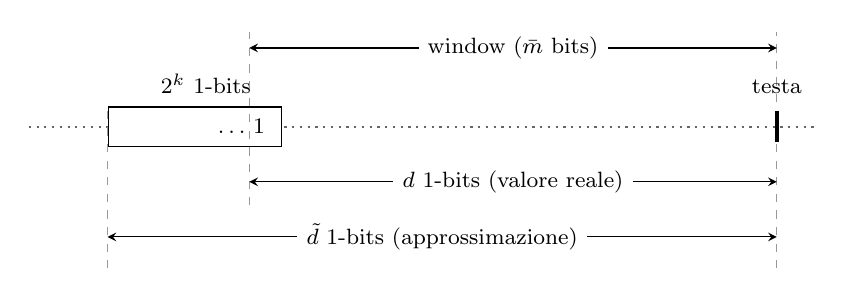
\begin{tikzpicture}[
        % Stili generali (font standard LaTeX)
        label/.style={font=\footnotesize},
        guide/.style={draw=black!40, dashed, thin},
        arrow/.style={stealth-stealth, thin},
        bucket/.style={draw=black, thin, fill=white}
    ]

    % 1. Linea temporale (bitstream punteggiato)
    \draw[black!60, dotted, thick] (-1, 0) -- (9, 0);

    % 2. Bucket più vecchio (2^k 1-bits) 
    % Posizionato tra x=0 e x=2
    \node[bucket, minimum width=2.2cm, minimum height=0.5cm, anchor=west] (oldbucket) at (0, 0) {};
    \node[label, anchor=south] at (1.25, 0.3) {$2^k$ 1-bits};
    \node[label] at (1.7, 0) {$\dots\,1$}; % L'ultimo "1" del bucket

    % 3. Marcatori verticali (Guide)
    \draw[guide] (0, -1.8) -- (0, 0.3);      % Fine del blocco (Inizio del valore reale d)
    \draw[guide] (1.8, -1.0) -- (1.8, 1.2);  % Inizio stima (e finestra m)
    \draw[guide] (8.5, -1.8) -- (8.5, 1.2);  % Head (Fine di tutto)

    % 4. Head
    \node[label, anchor=south] at (8.5, 0.3) {testa};
    \draw[ultra thick] (8.5, -0.2) -- (8.5, 0.2);

    % 5. Frecce (Allineate secondo le tue specifiche)
    
    % Window (m bits): Inizia dalla linea di stima (1.8) fino a head (8.5)
    \draw[arrow] (1.8, 1) -- (8.5, 1) node[midway, fill=white, label] {window ($\bar{m}$ bits)};

    % Valore reale d: Inizia dalla fine del blocco (0) fino a head (8.5)
    \draw[arrow] (1.8, -0.7) -- (8.5, -0.7) node[midway, fill=white, label] {$d$ 1-bits (valore reale)};

    % Approssimazione d_tilde: Stessa lunghezza della window (da 1.8 a 8.5)
    \draw[arrow] (0, -1.4) -- (8.5, -1.4) node[midway, fill=white, label] {$\tilde{d}$ 1-bits (approssimazione)};

    \end{tikzpicture}
    \label{DGIM_window}
\end{figure}